\chapter{Analysis}\label{ch:analysis}

The analysis process results in a model of the system that aims to be correct, complete, consistent and unambiguous \cite{bruegge2004object}. In this chapter, we focus on scenario-based analysis. Section \ref{requirements}, identifies the functional and nonfunctional requiremens of the system. In section \ref{system_models}, we describe a use case model that depicts the different interactions between the users and the system. Furthermore, we identify and study the objects of our system.


\section{Requirements}\label{requirements}

A requirement is a feature that the system must have or a constraint that it must satisfy to be accepted by the client \cite{bruegge2004object}. Requirements elicitation requires domain knowledge of the problem statement as well as experience in building software systems.

We design a system that uses synthetic and real images to classify different small parts. To do so, we create 3D models of our small parts. We subsequently generate a real image set for each small part, and a synthetic image set from the small part's 3D model. The real and synthetic image sets are combined to form a dataset, which we use to train a classification model based on convolutional neural networks. In this section we define the concrete functional and nonfunctional requirements needed to build our system.

\subsection{Functional Requirements}
Functional requirements (FRs) describe the interactions between the system and the its environment independent of its implementation \cite{bruegge2004object}.

The system's main function is to classify images of different small parts. Furthermore, the system needs to be dynamic and scalable to accomodate new small parts. To ensure that the system is able to classify images accurately, while leveraging synthetic input images, we introduce the following Functional Requirements.

\begin{itemize}
  \item [FR1] \textbf{Create 3D Model}: The system should use a 3D scanner to create a 3D model of a given small part.

  \item [FR2] \textbf{Generate Synthetic Image Set}: Given a 3D model of a small part, the system should place the 3D model in a synthetic scene and subsequently render a set of 2D synthetic images of the scene. The synthetic images should capture the 3D model in different positions.

  \item [FR3] \textbf{Set 3D Model Transformation Range}: To capture the model from different positions the model should be rotated and translated in the synthetic scene. The system should allow the user to define a rotation and transation range for each 3D model to avoid the risk of placing the 3D model in unrealistic positions.

  \item [FR4] \textbf{Generate Real Image Set}: Given a small part, the system should generate a set of real images of the small part.

  \item [FR5] \textbf{Split Input Dataset}: The synthetic and real image sets are combined to form a dataset. The system should split the dataset into a training set, a testing set and a validation set to train and evaluate a classification model. Moreover, the system should allow the user to set the ratio of synthetic to real images in the training set.

  \item [FR6] \textbf{Train Classification Model}: The system should have the capacity to train a classification model given a training and a validation set.

  \item [FR7] \textbf{Evaluate Classification Model}: The system should provide a mechanism to evaluate the performance of a given classification model.
\end{itemize}

\subsection{Nonfunctional Requirements}
Nonfunctional Requirements (NFRs) are key system requirements that apply to the system as a whole \cite{bruegge2004object}. To maintain the system's general requirements we define the following nonfunctional requirements.

\begin{itemize}
  \item [NFR1] \textbf{Performance}: A performence requirement is the measure of a quantifiable attribute of our system. In our case we would like to track our system's \textbf{classification accuracy}.
  \\We first define our system's accuracy for a single class to be the percentage of the given class's testing images that the classification model correctly predicts. We consequently define our system's classification accuracy to be the classification model's average prediction accuracy over each class.

  \item [NFR2] \textbf{Adaptability}: Adaptability is the ability to change a system to deal with additional application domain concepts \cite{bruegge2004object}. Our system should accomodate for the addition of new small parts to the set of target classes that our classification model is trained to identify. This addition can be done even after the system has been deployed.
\end{itemize}


\section{System Models}\label{system_models}

In this section we take a closer look at the system models. In section \ref{use_case_model}, we establish the main actors of our system and determine the actions that they can undertake. In section \ref{analysis_object_model}, we identify the objects of our system, we examine their behaviour and we study the relationship between them. Lastly, in section \ref{dynamic_model} we present activity diagrams that describe the workflows of our system.

\subsection{Use Case Model}\label{use_case_model}
Use case models represent the relationship between the user group of a system and the general functions that they can execute. A use case model can reduce the complexity of a system and increase its understandability.

The use case model of our system can be found as figure \ref{fig:UCM}. There are three main protagonists in our system. The \textit{3DModelCreator} is responsible for creating 3D models for the given small parts. The \textit{DataGenerator} uses the small parts and their corresponding 3D models to generate synthetic and real image sets. Finally, the \textit{MachineLearningEngineer} is responsible for creating a training, a validation and a testing sets. Moreover, the \textit{MachineLearningEngineer} trains the classification model to identify a set of small parts, and evaluates the model's performance.

The use case model can be divided into 4 main functions; namely creating 3D models, generating synthetic images, generating real images, and training/evaluating a classification model.

\begin{figure}[h]
\centering
  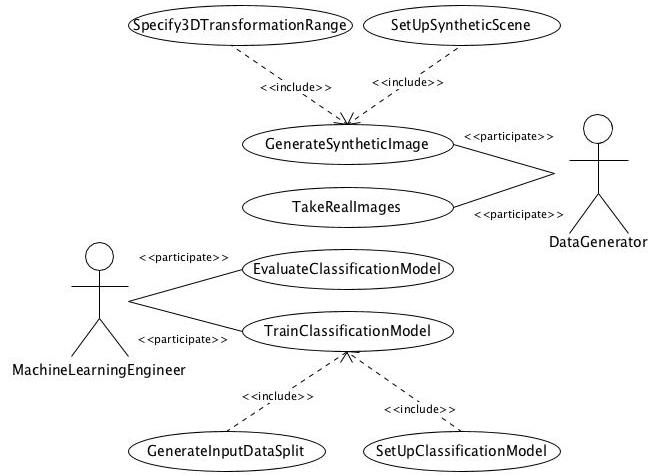
\includegraphics[width=\textwidth]{UCM}
\caption{The use case model displays the DataGenerator and the MachineLearningEngineer and the actions that they can undertake.}
\label{fig:UCM}
\end{figure}

\clearpage
\subsubsection{Creating 3D Models}
In order to create synthetic images, we need to create 3D models of our small parts. To do so, the 3DModelCreator uses a 3D scanner and compatible 3D scanning software to create the model.

\begin{usecase}
  \addtitle{Use Case}{Create3DModel}

  \addfield{Participating Actors}{3DModelCreator}

  \addscenario{Flow of Events}{
    \item The 3DModelCreator places the small part on a flat surface.
    \item The 3DModelCreator uses the 3D scanner to scan images of the small part from all directions.
    \item The 3D scanning software combines the scanned images to create a 3D model.
  }

  \additemizedfield{Entry Condition}{
    \item A small part has been chosen for scanning.
    \item The compatible 3D scanning software is open.
    \item The 3D scanner is turned on and recognized by the 3D scanning software.
  }

  \additemizedfield{Exit Condition}{
    \item A 3D model of the chosen small part has been created.
  }

  \additemizedfield{Quality Requirements}{
    \item The 3D model is as realistic as possible.
  }
\end{usecase}

\newpage
\subsubsection{Generating Synthetic Images}
Generating synthetic images the cornerstone for a synthetically augmented dataset. There's a lot of work that goes into generating the 3D synthetic scene and the corresponding renditions. Therefore, to increase the understandability of our model, we have separated the the use case that concerns modeling the 3D model as \textit{Specify3DTransformationRange}, and the use case that deals with the synthetic scene environment as \textit{SetUpSyntheticScene}.

\begin{usecase}
  \addtitle{Use Case}{Specify3DTransformationRange}

  \addfield{Participating Actors}{DataGenerator}

  \addscenario{Flow of Events}{
    \item In the modeling software, the DataGenerator chooses the transformations that are applicable to the small part's 3D model.
    \item For each transformation, the DataGenerator sets the range of each tranformation attribute that will be later used to generate a random position for the synthetic image of the small part.
  }

  \additemizedfield{Entry Condition}{
    \item A 3D model of a small part has been chosen.
  }

  \additemizedfield{Exit Condition}{
    \item All the transformation ranges for the 3D model have been set.
  }

  \additemizedfield{Quality Requirements}{
    \item The 3D transformation ranges should reflect the real-life transformations that the small parts can undergo.
    \item The 3D model should remain within camera viewfield.
  }
\end{usecase}

\newpage
\begin{usecase}
  \addtitle{Use Case}{SetUpSyntheticScene}

  \addfield{Participating Actors}{DataGenerator}

  \addscenario{Flow of Events}{
    \item In the modeling software, the DataGenerator places the 3D model of the small part on a horizontal plane as if lying on a table.
    \item The DataGenerator sets the background of the horizontal plane to mimic the background upon which the small part's real images are taken.
    \item The DataGenerator sets the lighting condition of the scene to reflect the lighting condition of the environment where the small part's real images are taken.
  }

  \additemizedfield{Entry Condition}{
    \item A 3D model of a small part has been chosen.
  }

  \additemizedfield{Exit Condition}{
    \item In the modeling software, the 3D model of the small part should be lying on a horizontal plane.
    \item The background and lighting condition should reflect the environment of the real image set.
  }

  \additemizedfield{Quality Requirements}{
    \item The synthetic scene should look as photorealistic as possible. This helps the classification model achieve a higher classification accuracy using the synthetic image set.
  }
\end{usecase}

\newpage
\begin{usecase}
  \addtitle{Use Case}{GenerateSyntheticImageSet}

  \addfield{Participating Actors}{DataGenerator}

  \addscenario{Flow of Events}{
    \item The DataGenerator specifies the desired number of output images in the synthetic image set.
    \item The modeling software generates the desired number of output synthetic images. Each image is a rendition of the synthetic scene after the transformations have been applied to the 3D model.
  }

  \additemizedfield{Entry Condition}{
    \item DataGenerator has set the transformation ranges of the 3D model.
    \item DataGenerator has set up the synthetic scene.
  }

  \additemizedfield{Exit Condition}{
    \item The DataGenerator obtains a set of synthetic images for the specified small part. The image set can be later used to train a classification model.
  }

  \additemizedfield{Quality Requirements}{
    \item The generated image dimensions should match the input dimensions required by the classification model.
  }
\end{usecase}

\newpage
\subsubsection{Generating Real Images}
The DataGenerator should strive to create an environment that is easy to model in 3D software. This will enable the creation of photo-realistic synthetic images.

\begin{usecase}
  \addtitle{Use Case}{GenerateRealImageSet}

  \addfield{Participating Actors}{DataGenerator}

  \addscenario{Flow of Events}{
    \item The DataGenerator places the camera over a plane.
    \item The DataGenerator sets the small part over the plane in a random position, while maintiaining that the small part remains horizontal. The full small part body should remain within the viewfield of the camera.
    \item The DataGenerator takes a picture of the small part.
    \item The DataGenerator repeats steps 2 and 3 until the desired number of real images of the small part is reached.
    \item The DataGenerator resizes the images to correspond to the input image size of the classification model. 
  }

  \additemizedfield{Entry Condition}{
    \item A small part has been chosen.
  }

  \additemizedfield{Exit Condition}{
    \item The DataGenerator obtains a set of real images for the specified small part that can be later used to train the classification model.
  }

  \additemizedfield{Quality Requirements}{
    \item The lighting of the environment should eliminate shadows and light reflections on the small part surface.
  }
\end{usecase}

\newpage
\subsubsection{Training the Classification Model}
The synthetic and real image sets are combined to form a dataset. Training a classification model requires the dataset to be split into a training, a validation, and a testing set. We model this requirement as the use case \textit{SplitInputDataset}. Furthermore the actions required for setting up the classification model are modeled as the use case \textit{SetUpClassificationModel}.

\begin{usecase}
  \addtitle{Use Case}{SplitInputDataset}

  \addfield{Participating Actors}{MachineLearningEngineer}

  \addscenario{Flow of Events}{
    \item The MachineLearningEngineer chooses the number of images for the training set, validation set and testing set.
    \item The MachineLearningEngineer chooses the ratio of synthetic images to real images in the training set.
  }

  \additemizedfield{Entry Condition}{
    \item For each small part set to be classified by the classification model, the corresponding real and synthetic image sets should be generated and ready for use.
  }

  \additemizedfield{Exit Condition}{
    \item The images in the dataset are split into a training, a validation and a testing set, ready to be used by the classification model.
  }
\end{usecase}

\newpage
\begin{usecase}
  \addtitle{Use Case}{SetUpClassificationModel}

  \addfield{Participating Actors}{MachineLearningEngineer}

  \addscenario{Flow of Events}{
    \item The MachineLearningEngineer chooses a convolutional neural network architecture for the classification model.
    \item The MachineLearningEngineer sets the hyperparameters: number of batches, number of epochs, number of frozen layers in the CNN, the optimizer and the hyperparameters associated with the chosen optimizer.
  }

  \additemizedfield{Exit Condition}{
    \item The classification model architecture, optimizer and corresponding hyperparameters should be selected.
  }
\end{usecase}

\newpage
\begin{usecase}
  \addtitle{Use Case}{TrainClassificationModel}

  \addfield{Participating Actors}{MachineLearningEngineer}

  \addscenario{Flow of Events}{
    \item The MachineLearningEngineer trains the classification model on the given training and validation sets.
    \item The MachineLearningEngineer evaluates the accuracy of the classification model by studying the model's predictions on the testing set.
    \item The MachineLearningEngineer fine-tunes the hyperparameters and re-trains the system until the maximum possible accuracy is reached.
  }

  \additemizedfield{Entry Condition}{
    \item The dataset should be split.
    \item The CNN model architecture, optimizer and initial hyperparameters should be chosen.
  }

  \additemizedfield{Exit Condition}{
    \item The classification model outputs the maximum possible accuracy given the input dataset.
  }

  \additemizedfield{Quality Requirements}{
    \item The classification model's hyperparameters should be fine-tuned until the maximum possible accuracy has been reached.
  }
\end{usecase}

\newpage
\subsection{Analysis Object Model}\label{analysis_object_model}
The analysis object model is a visual dictionary of the main concepts visible to the user \cite{bruegge2004object}. The analysis object model depicts a system's entites, their corresponding attributes and functions, and illustrates the relationship between said entitie. Figure \ref{fig:AOM} represents the analysis object model of our system.

\subsubsection{SmallPart}
A small part is the main subject of our system. It is an object that our system aims to classify. Each small part has a unique identifying label string.

\subsubsection{3DModel}
A 3DModel of a small part is the graphical model which helps our system create synthetic images. Each small part has a corresponding 3DModel. Each 3DModel has the same label as its small part counterpart.

\subsubsection{Transformation}
Each small part and 3DModel have a list of applicable transformations. A transformation is executed on an axis (x, y or z), and can either be a Translation or a Rotation.
At image generation time, each transformation outputs a random value between its defined maximum and minimum. We define a range to limit an object's transformation. For instance, we don't want to translate an small part so far as to remove it from the camera's viewfield.

\subsubsection{ImageGenerator}
ImageGenerator is the class that does the heavy lifting when it comes to creating images. It applies the random transformations on the target object and generates an image with a specified width and height.
ImageGenerator is an abstraction of 2 classes. SyntheticImageGenerator is responsible for applying the transformations on 3DModels, and using SyntheticScene to generate SyntheticImages, while RealImageGenerator uses a camera to take pictures of SmallMechanicalParts and output their corresponding RealImages.

\subsubsection{Image}
Image is a generalization of RealImage and SyntheticImage. Image stores information like width, height and label of the image. Moreover it contains a dataBuffer which contains the actual image pixel values.

\subsubsection{Dataset}
Dataset is a composition of Images. It is the image repository which is used by the ImageClassifier for training and evaluation.

\subsubsection{DataSplitGenerator}
DataSplitGenerator splits the Dataset into a training set, validation set and testing set. This split prepares the data for consumption by the ImageClassifier.

\subsubsection{CNNModel}
CNNModel is the convolutional neural network algorithm that is trained for image classification. CNNModel is an abstraction of 4 different CNN architectures, namely Inception, Resnet, VGG16 and VGG19. Furthermore, CNNModel defines the weights that are used to initialize the CNN to leverage the power of transfer learning. CNNModel also sets the number of trainable layers in a network to potentially preserve the initial weights and speed up training.

\subsubsection{Optimizer}
Each CNNModel has an Optimizer. An Optimizer is the function aims to close the gap between the model's predictions of the validation set labels and their corresponding ground truth. The Optimizer operates in the CNNModel's training phase. Optimizer is an abstraction of 2 different optimizers that we use in our system. Specifically SGD (Stochastic Gradient Descent), and Adam.

\subsubsection{ImageClassifier}
ImageClassifier orchestrates the feeding of data into the CNNModel for training. Moreover, it uses the testing set to calculate the accuracy of the trained model.

\begin{figure}[H]
\centering
  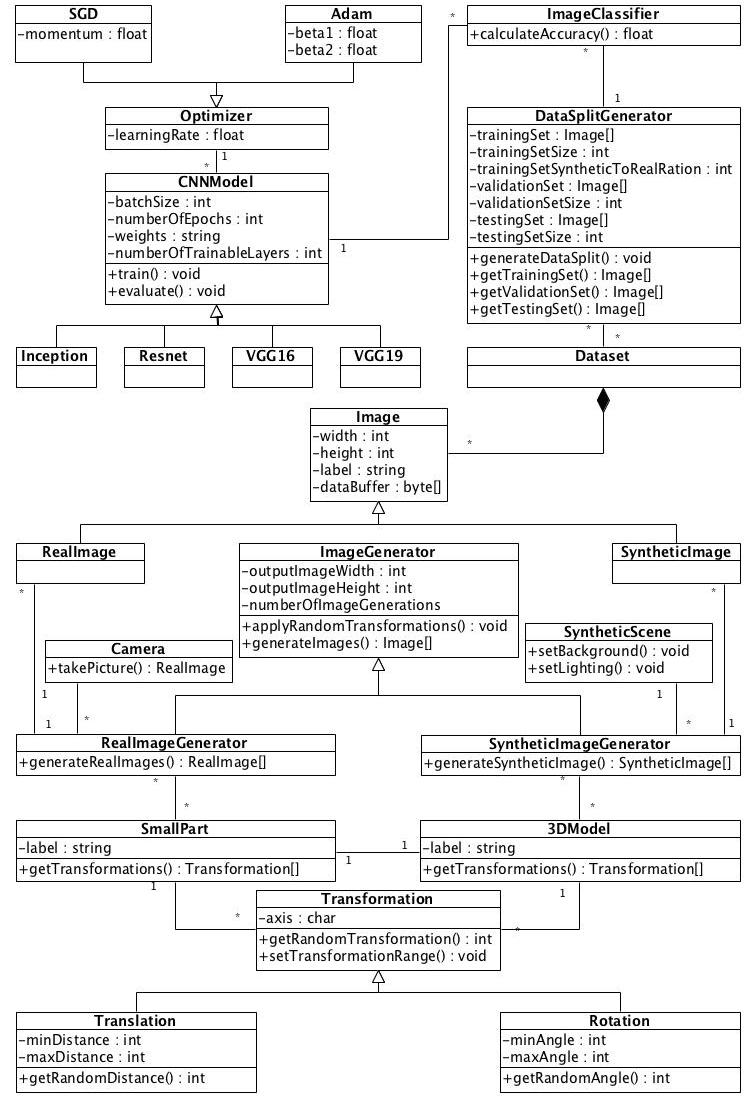
\includegraphics[width=\textwidth]{AOM}
\caption{The analysis object model of our system identifies our system's objects as well as their attributes and functions.}
\label{fig:AOM}
\end{figure}

\subsection{Dynamic Model}\label{dynamic_model}
The dynamic model is focused on the behavior of the system. Sequence diagrams, activity diagrams and state machines are usually used to depict dynamic models \cite{bruegge2004object}. In this section we present 3 activity diagrams, each depicts a workflow in our system. Namely, the workflow to create a real image set from a small part, the workflow to create the small part's 3D model and subsequently generate the synthetic image set of the small part, and the workflow to train a classification model using both image sets.

\subsubsection{Dataset Generation}
Figure \ref{fig:AD1} depicts the workflow of activities required to generate a dataset. The DataGenerator selects a small part and its corresponding 3D model. The DataGenerator then proceeds to generate the real and synthetic images. Finally the images are combined to form a dataset.

\begin{figure}[H]
\centering
  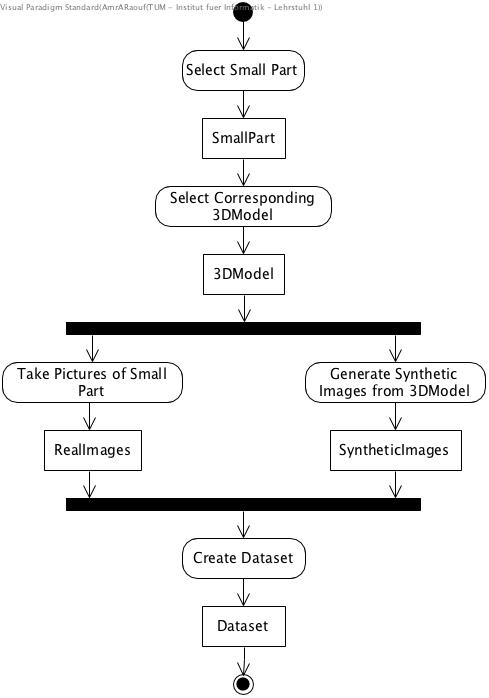
\includegraphics[width=0.65\textwidth]{AD1}
\caption{Activity Diagram depicting the workflow required for Dataset generation.}
\label{fig:AD1}
\end{figure}

\subsubsection{Obtain Image Classifier}
Figure \ref{fig:AD2} describes the workflow of activities required to obtain the image classifier. The MachineLearningEngineer splits the data into training, validation and testing sets. The MachineLearningEngineer then creates a CNN model. Next the MachineLearningEngineer feeds the training data to the CNN model to obtained a trained CNN model. The MachineLearningEngineer then evaluates the trained CNN model accuracy using the testing set. If the accuracy of the trained CNN model is not sufficient, the CNN model is fine tuned and re-trained.

\begin{figure}[H]
\centering
  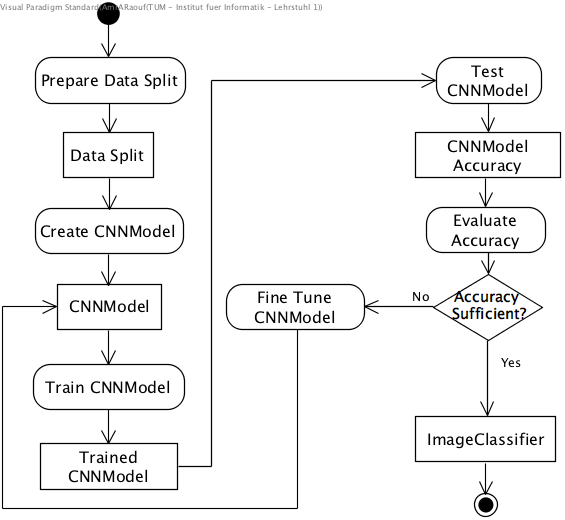
\includegraphics[width=0.7\textwidth]{AD2}
\caption{Activity Diagram describing the workflow required to obtain the Image Classifier.}
\label{fig:AD2}
\end{figure}
